\documentclass[10pt,twocolumn,a4paper]{ctexart}
\usepackage[margin=1.7cm,columnsep=0.65cm]{geometry}
\usepackage{amsmath,amssymb,bm}
\usepackage{booktabs}
\usepackage{graphicx}
\usepackage{microtype}
\usepackage{natbib}
\usepackage{xcolor}
\usepackage{hyperref}
\usepackage{enumitem}
\usepackage{fancyhdr}
\usepackage{float}

\graphicspath{{../../artifacts/figures/}}
\renewcommand{\topfraction}{0.9}\renewcommand{\dbltopfraction}{0.9}
\renewcommand{\textfraction}{0.07}\renewcommand{\floatpagefraction}{0.75}
\renewcommand{\dblfloatpagefraction}{0.75}\setcounter{topnumber}{3}\setcounter{dbltopnumber}{2}
\setlength{\parindent}{2em}
\setlist{nosep,leftmargin=*}
\hypersetup{colorlinks=true,linkcolor=blue!55!black,
  citecolor=green!45!black,urlcolor=blue!65!black}
\pagestyle{fancy}
\fancyhf{}
\fancyhead[L]{CS224R 2025 Homework 3}
\fancyhead[R]{ShaneLiu04}
\fancyfoot[C]{\thepage}

\newcommand{\figmaybe}[2]{%
  \IfFileExists{../../artifacts/figures/#1.png}{%
    \includegraphics[width=\linewidth]{#1}}{%
    \fbox{\parbox[c][3.2cm][c]{\linewidth}{\centering\small #2}}}}

\title{\vspace{-1.2em}\textbf{探索数据上的离线强化学习：\\
IQL 的 expectile、CQL 的保守性与数据来源}}
\author{ShaneLiu04\\
\small\url{https://github.com/ShaneLiu04}}
\date{}

\begin{document}
\maketitle
\thispagestyle{fancy}

\begin{abstract}
本文完成 CS224R 2025 Homework 3：在 PointMass 迷宫上实现 Implicit Q-Learning（IQL）与
离散动作 Conservative Q-Learning（CQL），比较 Random Network Distillation（RND）与均匀
随机两种无监督探索得到的数据。IQL 在 Easy 上 $\zeta=0.9$ 的回报为 $-18.8\pm0.5$，优于
$\zeta=0.2$ 的 $-20.4\pm0.8$（各 $6$ 个种子）；Medium 上 RND 数据比随机数据高约
$30$--$40$。CQL 在 Medium 上 $\alpha=0$ 的全部种子停在 episode 上限 $-150$，
$\alpha=0.1$ 为 $-68.5\pm11.5$。核对 starter 后我们发现，CQL 的数据采集在两种探索设定下
都调用同一个最短路贪心控制器，因此作业里 CQL 的 ``RND 对 random'' 对比实际上比较的是
同一份专家数据。我们补充了该控制器的回报（$-67.2$）、$\alpha$ 的七点扫描与分布外
间隙，并新增 \texttt{--behavior explore} 让 CQL 真正使用探索数据：在均匀随机数据上
$\alpha=0.1$ 达到 $-34.3\pm6.1$，明显超过专家控制器本身。
\end{abstract}

\textbf{关键词：}Offline RL；IQL；CQL；Expectile；RND；Exploration Data；Coverage

\section{问题与设定}
PointMass 是带墙的二维迷宫，$5$ 个离散动作（四个方向与不动），动作带高斯噪声；
到达目标得 $0$，其余每步 $-1$，episode 上限 Easy $50$、Medium $150$、Hard $100$ 步。
因此 $-150$ 表示在 Medium 上始终没有到达目标。

一次运行共 $5\times10^4$ 个环境步，分为探索与利用两段\citep{yarats2022exorl}。
探索阶段只优化内在奖励。RND 固定随机目标网络 $f^*$，训练预测网络 $\hat f$，用
$\lVert\hat f(s')-f^*(s')\rVert$ 作奖励\citep{burda2019rnd}；随机探索在
\texttt{learning\_starts} 之前全部均匀采样动作。利用阶段用环境奖励训练离线 critic：
\begin{itemize}
\item IQL 按作业命令运行，探索 $2\times10^4$ 步。命令没有 \texttt{--offline\_exploitation}，
所以利用阶段仍以 $\varepsilon=0.2$ 继续写入缓冲区，严格说是 offline-to-online。
\item CQL 带 \texttt{--offline\_exploitation}，探索 $10^4$ 步（starter 默认值）后缓冲区冻结，
是严格的离线设定。
\end{itemize}

\section{方法}
\subsection{IQL}
IQL 只在数据动作上做备份\citep{kostrikov2022iql}：
\begin{align}
L_V&=\mathbb{E}_{\mathcal{D}}\bigl[L_2^\zeta(\bar Q(s,a)-V(s))\bigr],\quad
L_2^\zeta(u)=|\zeta-\mathbb{1}(u<0)|u^2,\\
L_Q&=\mathbb{E}_{\mathcal{D}}\bigl[(r+\gamma(1-d)V(s')-Q(s,a))^2\bigr].
\end{align}
$\bar Q$ 来自目标网络并 detach。策略用 AWAC 的优势加权对数似然抽取，
$A=Q(s,a)-V(s)$ 在无梯度下计算并压成形状 $(N,)$\citep{nair2020awac,peng2019awr}。
$\zeta=0.5$ 时 $V$ 是行为策略价值；$\zeta\to1$ 时逼近数据支撑内的 $\max_a Q$
\citep{newey1987expectile}。

\subsection{CQL}
离散动作下 CQL 正则可以精确计算\citep{kumar2020cql}：
\begin{equation}
\mathcal{L}=\mathcal{L}_{\mathrm{DQN}}+\alpha\,\mathbb{E}_{s,a\sim\mathcal{D}}
\Bigl[\log\textstyle\sum_{a'}e^{Q(s,a')}-Q(s,a)\Bigr].
\end{equation}
实现用 \texttt{torch.logsumexp}，同时记录 $\log\sum e^{Q}$ 与 $Q(s,a_{\mathcal{D}})$，
二者之差称为分布外间隙（OOD gap）。官方单元测试输出 \texttt{PASSED!!}，我们另写了
$5$ 个 pytest 用例核对 IQL 的 expectile、$V$/$Q$ 目标与 CQL 正则。

\subsection{数据采集器的发现与修正}
starter 的 \texttt{ExplorationOrExploitationAgent.step\_env} 把探索策略的代码注释掉，
每一步都执行 \texttt{env.get\_optimal\_action(env.state)}：在一步仿真后选择最短路
距离（全源最短路）最小的动作。因此 CQL 的 \texttt{--use\_rnd} 只改变
\texttt{learning\_starts}（$2000$ 或 $10^4$），不改变数据。图~\ref{fig:traj} 中三组 CQL
的状态密度图完全相同，也印证了这一点。我们在 solutions 副本中增加
\texttt{--behavior \{oracle,explore\}}：默认 \texttt{oracle} 与 starter 完全一致；
\texttt{explore} 恢复与 IQL agent 相同的采集逻辑（$\varepsilon$-greedy 地执行探索
critic 的 argmax，\texttt{learning\_starts} 之前均匀随机）。另写
\texttt{analysis/oracle\_baseline.py} 评估该控制器本身：Easy $-18.4$、Medium $-67.2$、
Hard $-55.9$（各 $20$ 条 episode，成功率 $1.0/1.0/0.95$）。

\subsection{实验}
所有配置至少 $3$ 个种子，作业要求的配置 $6$ 个种子。最终回报取每个种子最后 $3$ 次评估
的均值，再报告跨种子均值 $\pm$ 标准差（总体标准差）。运行在 CPU 上并行完成，
曲线由 TensorBoard 事件导出。

\section{IQL}
\begin{figure}[H]
\centering
\figmaybe{hw3_fig1_iql_expectile}{IQL expectile}
\caption{PointmassEasy 上的 expectile 扫描。左：评估回报曲线，虚线为探索结束。
右：最终回报，黑点为单个种子。}
\label{fig:zeta}
\end{figure}

\paragraph{Q1.1：$\zeta=0.2$ 与 $0.9$。}Easy 上 $\zeta=0.9$ 的最终回报为
$-18.84\pm0.48$，$\zeta=0.2$ 为 $-20.36\pm0.81$（各 $6$ 个种子），中间的 $0.5$ 与 $0.7$
分别为 $-19.71$ 与 $-18.71$（图~\ref{fig:zeta}）。较大的 $\zeta$ 更好：$V(s)$ 拟合数据中
$Q$ 的上分位，近似“数据支撑内最好的动作”的价值，优势 $Q-V$ 只对优于大多数数据动作的
动作为正，AWR 的权重因此集中在更好的动作上。$\zeta=0.2$ 则让 $V$ 低于平均，几乎所有
动作的优势为正，策略抽取接近行为克隆。Easy 迷宫很小，RND 数据已覆盖目标，所以差距只有
约 $1.5$；对照专家控制器的 $-18.4$，$\zeta\ge0.7$ 已接近最优。

\begin{figure}[H]
\centering
\figmaybe{hw3_fig2_iql_exploration}{IQL exploration}
\caption{PointmassMedium 上 RND 与随机探索数据（各 $6$ 个种子）。}
\label{fig:iqlexp}
\end{figure}

\begin{table}[H]
\centering
\caption{IQL 在 PointmassMedium 上的最终回报（$6$ 个种子）。}
\label{tab:iql}
\begin{tabular}{lcc}
\toprule
 & RND & random \\
\midrule
$\zeta=0.7$ & $-50.9\pm2.4$ & $-90.7\pm6.7$ \\
$\zeta=0.9$ & $-59.7\pm36.9$ & $-89.8\pm15.8$ \\
\bottomrule
\end{tabular}
\end{table}

\paragraph{Q1.2：RND 与 random。}表~\ref{tab:iql} 与图~\ref{fig:iqlexp} 中，两种 $\zeta$ 下
RND 都比随机探索高 $30$ 以上。$\zeta=0.9$ 的 RND 有一个种子停在 $-141.6$，其余五个在
$-38$ 到 $-50$ 之间，均值因此被拉低、方差很大；$\zeta=0.7$ 的六个种子都在 $-48$ 到
$-55$，更稳定。曲线显示随机数据上的 IQL 在探索结束（$2\times10^4$ 步）时仍为 $-150$，
之后靠利用阶段的在线数据才慢慢上升；RND 数据上回报在探索阶段就开始上升。
这说明在 offline RL 中，数据决定了可学的上限：均匀随机游走的扩散半径随 $\sqrt{t}$ 增长，
状态密度集中在起点附近（图~\ref{fig:traj} 第二行），远端走廊和目标附近几乎没有转移；
RND 主动访问预测误差大的状态，覆盖了通往目标的路径。IQL 只在数据动作上备份，没有
数据的区域无法通过外推补上\citep{schweighofer2022dataset,jin2021pessimism}。

\paragraph{补充扫描。}Medium 上 RND 数据的 $\zeta=0.5,0.7,0.9,0.95$ 分别为
$-98.1\pm32.1$、$-50.9\pm2.4$、$-59.7\pm36.9$、$-47.8\pm11.2$（图~\ref{fig:sweeps} 右）。
$\zeta=0.5$ 即 SARSA 式的行为价值，明显最差；$0.7$ 以上差别在种子噪声内，高 $\zeta$
的方差更大，因为 $V$ 依赖少数高价值样本。Hard 上 $\zeta=0.9$ 只有 $-93.3\pm3.8$，
低于专家控制器的 $-55.9$。

\section{CQL}
\begin{figure}[H]
\centering
\figmaybe{hw3_fig3_cql_alpha}{CQL alpha}
\caption{CQL 在 PointmassMedium 上的评估回报。左：$\alpha$；右：两种探索标志。}
\label{fig:cqlalpha}
\end{figure}

\paragraph{Q2.1：$\alpha=0$ 与 $0.1$。}$\alpha=0$ 时正则消失，算法退化为在固定缓冲区上训练的
double DQN。六个种子的最终回报全部为 $-150$；$\alpha=0.1$ 为 $-68.5\pm11.5$（逐种子
$-63.5,-83.9,-49.8,-74.7,-77.6,-61.3$）。图~\ref{fig:qvals} 给出原因：$\alpha=0$ 时数据
动作的 Q 值约为 $-1.0$，$\log\sum e^{Q}$ 为 $0.91$，间隙 $1.91$。每步奖励为 $-1$、到达目标
需要几十步，真实价值远低于 $-1$，这是典型的过估计。数据由专家控制器采集，每个状态几乎
只出现一个动作；$\max_{a'}Q(s',a')$ 总会挑到没有被数据约束的动作，误差经备份传回
\citep{fujimoto2019bcq,kumar2019bear}。贪心策略于是执行这些虚高的动作，在迷宫里卡住。
$\alpha=0.1$ 时数据 Q 降到 $-12.7$，间隙降到 $0.48$，策略回到专家动作附近。

\begin{figure*}[!t]
\centering
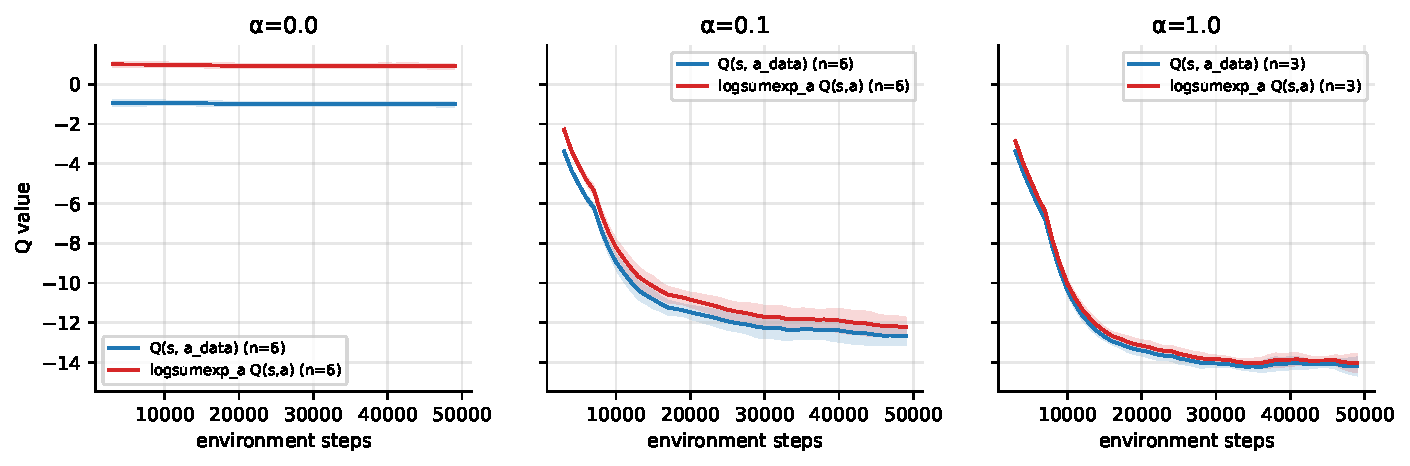
\includegraphics[width=0.85\linewidth]{hw3_fig4_cql_qvalues}
\caption{CQL 的 $Q(s,a_{\mathcal{D}})$ 与 $\log\sum_a e^{Q(s,a)}$。$\alpha=0$ 时分布外动作的
软最大值高于数据动作，Q 值接近 $-1$，远高于真实回报。}
\label{fig:qvals}
\end{figure*}

\begin{figure}[H]
\centering
\figmaybe{hw3_fig6_medium_sweeps}{sweeps}
\caption{左：CQL $\alpha$ 七点扫描的最终回报（蓝）与分布外间隙（红，右轴）。
右：IQL $\zeta$ 扫描。}
\label{fig:sweeps}
\end{figure}

\paragraph{$\alpha$ 扫描。}图~\ref{fig:sweeps} 左：$\alpha=0.01,0.03,0.1,0.3,1,3$ 的回报分别为
$-72.5,-59.3,-68.5,-61.8,-66.6,-67.0$，间隙从 $0.98$ 单调降到 $0.12$。只要
$\alpha>0$，策略就不再崩溃；$\alpha\ge0.3$ 后方差很小，回报稳定在专家控制器的
$-67.2$ 附近。这符合 CQL 的理论：$\alpha$ 越大，学到的 Q 越接近行为策略的价值下界，
策略越接近行为策略\citep{kumar2020cql}。小 $\alpha$（$0.01$）有一个种子跌到 $-117$，
保守性不足时外推仍会偶发。Hard 上同样，$\alpha=0$ 停在上限 $-100$，$\alpha=0.1$ 为
$-41.1\pm2.0$，高于专家控制器的 $-55.9$：控制器的一步前瞻没有考虑动作噪声，
在窄通道附近并非最优，CQL 在其数据附近做了小幅的策略改进。

\paragraph{Q2.2：RND 与 random 标志。}按作业命令，$\alpha=0.1$ 时 RND 标志为
$-68.5\pm11.5$，random 标志为 $-60.2\pm5.8$（各 $6$ 个种子），差别在种子噪声内。原因是
上节的发现：两个标志下数据完全相同，只是 random 标志把 critic 的训练起点推迟到第
$10^4$ 步。图~\ref{fig:traj} 中 CQL 三行的状态密度一致，轨迹集中在专家路径上。

\section{CQL 真正使用探索数据时}
\begin{figure*}[!t]
\centering
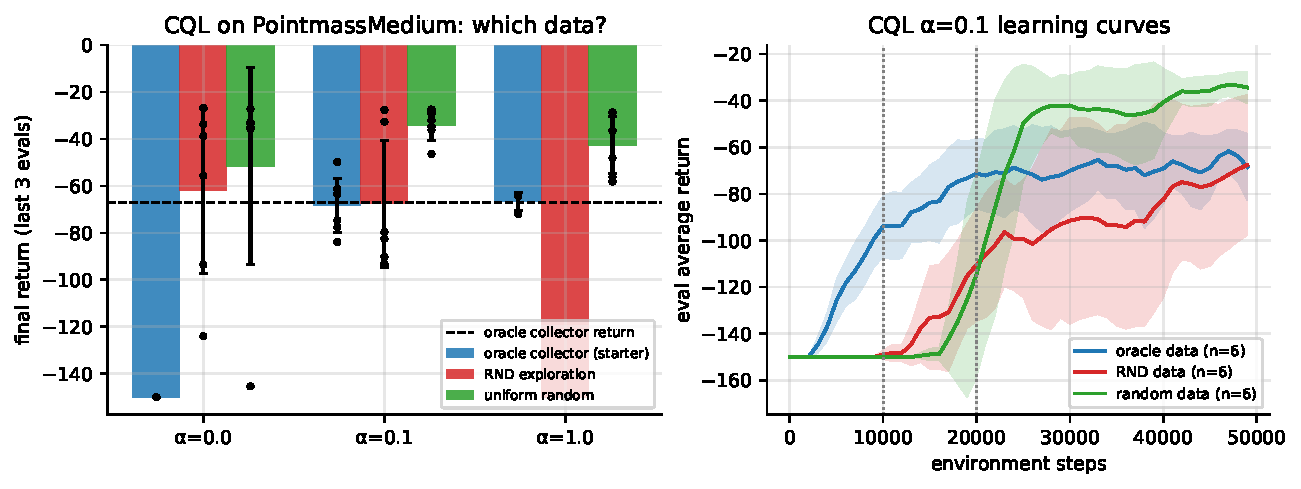
\includegraphics[width=0.9\linewidth]{hw3_fig8_cql_data_source}
\caption{PointmassMedium 上三种数据来源的 CQL（\texttt{--behavior explore} 各 $6$ 个种子）。
虚线为专家控制器的回报 $-67.2$。右：$\alpha=0.1$ 的学习曲线，两条竖线分别为
CQL 的探索结束（$10^4$）与 IQL 的探索结束（$2\times10^4$）。}
\label{fig:source}
\end{figure*}

\begin{table}[H]
\centering
\caption{CQL 在 PointmassMedium 上按数据来源的最终回报。}
\label{tab:source}
\small
\begin{tabular}{lccc}
\toprule
数据 & $\alpha=0$ & $\alpha=0.1$ & $\alpha=1$ \\
\midrule
专家（starter） & $-150.0\pm0.0$ & $-68.5\pm11.5$ & $-66.6\pm3.7$ \\
RND 探索 & $-62.1\pm35.3$ & $-67.6\pm26.9$ & $-150.0\pm0.0$ \\
均匀随机 & $-51.6\pm42.0$ & $-34.3\pm6.1$ & $-42.7\pm12.1$ \\
\bottomrule
\end{tabular}
\end{table}

表~\ref{tab:source} 与图~\ref{fig:source} 给出三点结论。

第一，数据的动作覆盖决定了是否需要保守。专家数据上 $\alpha=0$ 必然崩溃；探索数据
在每个状态上覆盖多个动作，$\max_{a'}$ 查询的动作大多有数据约束，即使 $\alpha=0$ 的
离线 DQN 也能学到 $-50$ 到 $-60$ 的策略，只是方差很大（随机数据有一个种子为 $-145$）。
这与 ExORL 的观察一致：在探索性数据上，普通的 off-policy 算法已经可以工作
\citep{yarats2022exorl}。

第二，覆盖面广的数据让 CQL 超过专家。均匀随机数据上 $\alpha=0.1$ 达到
$-34.3\pm6.1$，六个种子都优于专家控制器的 $-67.2$。专家数据只沿一条路径，CQL 只能在
其附近改进；随机数据虽然质量低，但包含大量不同动作的转移，动态规划可以把片段拼成更短的
路径\citep{kumar2022should}。

第三，保守性会把策略拉向行为策略，行为策略的偏差因此变得重要。RND 数据上 $\alpha=1$
的六个种子全部为 $-150$。RND 的探索策略在后期主要执行探索 critic 的 argmax，
动作分布偏向“去新奇的地方”而不是“去目标”；$\alpha$ 很大时 CQL 近似对行为策略做加权
模仿，学到的是探索行为。均匀随机数据的动作分布对称，同样的 $\alpha=1$ 只把 Q 整体
下压，不偏向任何动作，所以仍有 $-42.7$。这一对比说明 $\alpha$ 的合适取值依赖数据的
行为策略：数据越接近专家，越需要保守；数据越偏离任务，越不能过度保守。

这一组结果也与 IQL 的 Q1.2 方向不同：IQL 在 RND 数据上更好，CQL 在随机数据上更好。
两者的设定不同。IQL 探索 $2\times10^4$ 步且之后继续在线收集，CQL 只用 $10^4$ 步的冻结数据；
$10^4$ 步内随机探索在 Medium 上已能偶尔到达目标附近，而 RND 的 argmax 探索策略的动作
多样性低于均匀随机。数据的``好坏''不能脱离算法与预算单独讨论。

\begin{figure}[H]
\centering
\figmaybe{hw3_fig5_trajectories}{trajectories}
\caption{各设定种子 $0$ 的探索状态密度（左）与最终评估轨迹（右）。IQL 两行的密度不同；
CQL 三行（starter 采集器）的密度完全相同。}
\label{fig:traj}
\end{figure}

\begin{figure}[H]
\centering
\figmaybe{hw3_fig7_hard}{hard}
\caption{PointmassHard：IQL 与 CQL（starter 采集器），虚线为采集器自身回报。}
\label{fig:hard}
\end{figure}

\section{结论}
IQL 的 expectile 越高，策略抽取越接近数据支撑内的贪心改进，Easy 上 $\zeta=0.9$ 优于
$0.2$；Medium 上 RND 数据比随机数据高 $30$ 以上，差距来自数据覆盖。CQL 的
$\alpha=0$ 在专家数据上因分布外动作过估计而完全失败，任意 $\alpha>0$ 都能恢复到
专家水平。作业中 CQL 的 RND/random 对比被 starter 的固定采集器消解；修正后，均匀随机
数据上的 CQL 显著超过专家，而 RND 数据配合大 $\alpha$ 会模仿探索行为而失败。
离线 RL 的结果是算法、保守系数与数据行为策略三者的乘积，不能只讨论其中一项。

\clearpage
\bibliographystyle{plainnat}
\bibliography{../references}

\end{document}
